\documentclass[onecolumn, draftclsnofoot,10pt, compsoc]{IEEEtran}
\usepackage{graphicx}
\usepackage{url}
\usepackage{setspace}
\usepackage{pgfgantt}

\newcommand{\indentitem}{\setlength\itemindent{35pt}}

\newcommand{\subsubsubsection}[1]{\paragraph{#1}\mbox{}\\}
\setcounter{secnumdepth}{5}
\setcounter{tocdepth}{5}
\setlength\parindent{0pt}


\usepackage{geometry}
\geometry{textheight=9.5in, textwidth=7in}
\title{Requirements Document}
% 1. Fill in these details
\def \CapstoneTeamName{		Team PHAZE}
\def \CapstoneTeamNumber{		53}
\def \GroupMemberOne{			Alessandro Lim}
\def \GroupMemberTwo{			Touku Cha}
\def \GroupMemberThree{			Jaydeep Rotithor}
\def \CapstoneProjectName{		PHAZE | IoT Weather Station}
\def \CapstoneSponsorCompany{		Openly Published Environmental Sensing Lab}
\def \CapstoneSponsorPerson{		Chet Udell}

% 2. Uncomment the appropriate line below so that the document type works
\def \DocType{		%Problem Statement
				Requirements Document
				%Technology Review
				%Design Document
				%Progress Report
				}
			
\newcommand{\NameSigPair}[1]{\par
\makebox[2.75in][r]{#1} \hfil 	\makebox[3.25in]{\makebox[2.25in]{\hrulefill} \hfill		\makebox[.75in]{\hrulefill}}
\par\vspace{-12pt} \textit{\tiny\noindent
\makebox[2.75in]{} \hfil		\makebox[3.25in]{\makebox[2.25in][r]{Signature} \hfill	\makebox[.75in][r]{Date}}}}
% 3. If the document is not to be signed, uncomment the RENEWcommand below
%\renewcommand{\NameSigPair}[1]{#1}

%%%%%%%%%%%%%%%%%%%%%%%%%%%%%%%%%%%%%%%
\begin{document}
\begin{titlepage}
    \pagenumbering{gobble}
    \begin{singlespace}
    	
\includegraphics[height=4cm]{coe_v_spot1}
        \hfill 
        % 4. If you have a logo, use this includegraphics command to put it on the coversheet.
        %\includegraphics[height=4cm]{CompanyLogo}   
        \par\vspace{.2in}
        \centering
        \scshape{
            \huge CS Capstone \DocType \par
            {\large\today}\par
            \vspace{.5in}
            \textbf{\Huge\CapstoneProjectName}\par
            \vfill
            {\large Prepared for}\par
            \Huge \CapstoneSponsorCompany\par
            \vspace{5pt}
            {\Large\NameSigPair{\CapstoneSponsorPerson}\par}
            {\large Prepared by }\par
            Group\CapstoneTeamNumber\par
            % 5. comment out the line below this one if you do not wish to name your team
            \CapstoneTeamName\par 
            \vspace{5pt}
            {\Large
                \NameSigPair{\GroupMemberOne}\par
                \NameSigPair{\GroupMemberTwo}\par
                \NameSigPair{\GroupMemberThree}\par
            }
            \vspace{20pt}
        }
        \begin{abstract}
                % 6. Fill in your abstract   
        Due to the low-cost nature of microcontrollers such as the Feather MO, we are able to connect various sensors to them to create a miniature weather station.
        Using the concept of Internet of things, we are able to connect multiple weather stations together to measure data across a wide area.
        The data is transferred over long distances using LoRa radios and uploaded to the cloud.
        Once the data is available on the cloud researchers can access the data from anywhere in the world, and change it on the fly
        \end{abstract}     
    \end{singlespace}
\end{titlepage}
\newpage
\pagenumbering{arabic}
\tableofcontents
% 7. uncomment this (if applicable). Consider adding a page break.
%\listoffigures
%\listoftables
\clearpage

% 8. now you write!
\section{Introduction}
\subsection{Purpose}
The purpose of this document is to describe the requirements for the Internet of Things Weather station. It will give an overview of the project and go over its various aspects. It will then discuss assumptions and limitations for the project, and then give an in-depth description of the requirements for our finished product. This document has been created as a reference for our client and as a guide for what our final product should look like.
\subsection{Scope}
PHAZE is an evaporometer which measures environmental data. The device will be used to help researchers gather weather information from remote areas, such as the H.J. Andrews Forest. The device will measure temperature, humidity, albedo, and rainfall. It is also built to protect the microcontrollers from humidity. 


At least 20 PHAZE devices are planned to be deployed. The devices will transmit the data with LoRa radios to a server. The data from the devices will be handled by the server and will be uploaded. The data will be available in Google Drive and will be visualized in the OSU GeoViz system. 

\subsection{Definitions, acronyms and abbreviations}
\begin{itemize}
\item Database: a collection of data stored on the Internet.
\item Evaporometer: The weather collecting device we will be building.
\item GeoViz: A Geo-visualization hosted on a website.
\item Google Drive: A cloud storage hosted by Google.
\item IDE: an integrated development environment is a software application used in software development.
\item IoT: internet of things, the connection of devices via the Internet to transmit and receive data.
\item LoRa: long range, low power wireless radio.
\item Microcontroller: a small computer on a single circuit.

\item SD: secure digital, a non-volatile memory card used in the Evaporometer.


\end{itemize}
\subsection{Reference}
Images courtesy of:
\begin{itemize}
\item https://learn.Adafruit.com
\item https://iotdk.intel.com
\item https://store.open-electronics.org
\item http://geoviz.ceoas.oregonstate.edu/
\end{itemize}

\section{Overall Description}
This section will go over the whole project.  The project consists of multiple parts that interact with each other over the Internet.  It will describe how each parts operates with each other to accomplish the task of collecting data and converting it to real world values for researchers to use.
\subsection{Product Perspective}
The parts of the project are: data collection, data transfer, and one web portal.  The evaporometers are set up ahead of time and deployed into an environment.
\newline
\begin{figure}
 \caption{How the sensor and microcontroller connection is set.}
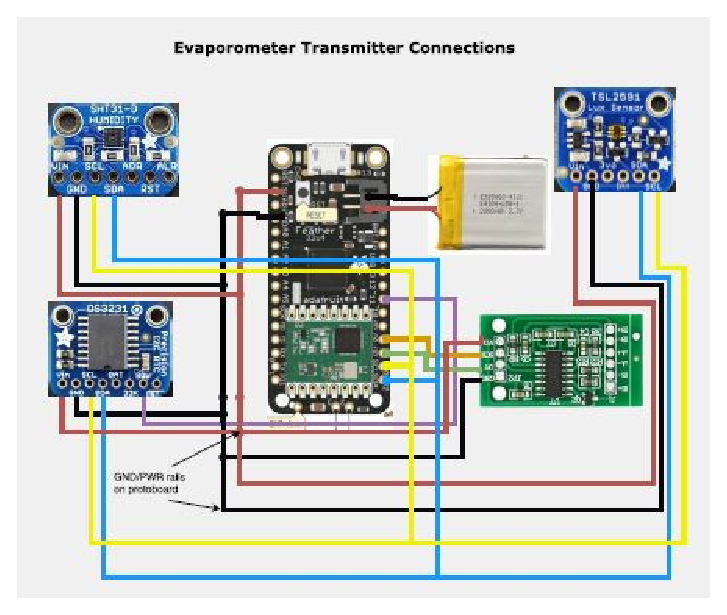
\includegraphics{connections.eps}
\end{figure}


The devices are enclosed in a 3D printed enclosure and are programmed in the Arduino IDE with the sensors attached.  Each device is pre-programmed to wake up every five minutes to collect data with the installed sensors.  After data collection has finished each device will save the information onto it’s SD card before transmitting the data.  This is to ensure that data can still be retrieved after power loss or packets being dropped during transfer.
\newline

After the data is saved onto the SD card the devices will transmit all collected data to the LoRa hub.  The LoRa hub will check to make sure all collected data are transferred correctly.  Due to the environment, packets can be dropped causing the data to be corrupted.  If data is missing or corrupt the LoRa will ping the device to collect/transfer data again until a predetermined stop signal.  This will prevent the devices from continually collecting data if it’s sensors are damaged and stop the hub from asking for more data from a dead device.
\newline

Once data collection is finished the hub will begin the transfer process.  The hub will upload the data to the OPEnS Google Drive to hold all collected information via ethernet.  The data will be available in datasheets and can be easily transferred to other databases for usage.
\newline

We will be using the data analytics and visualization tool, GeoViz, to visualize all of our data.  The data will used to create geographical graph for researchers to use.  The visuals can be updated on the fly with additional data collected over time.
\subsection{Product Functions}
With the data up on GeoViz, researchers can view the data from anywhere in the world.  Researchers can always view the most current data by viewing the database.  If needed the researchers can travel to each device and collect the data straight from the SD card.


Each device can be setup to accommodate various sensors and will be rechargeable via solar panels.  If a hard reset is necessary a physical reset button is attached to the device for researchers to press, versus opening up the entire enclosure.
\subsection{User Characteristics}
The users that will use the device are researchers. They will not interact with the hardware. However, they will interact with the data measured by the device. Which will be available on Google Drive and GeoViz.
\subsection{Constraints}
The Internet connection is a constraint for the server. If the internet connection in the server is cut off, the server will be unable to upload any data to Google Drive and the GeoViz.


Cloud storage space is also a constraint to the project. Google Drive is the main storage of the project. Once the max capacity of Google Drive is reached, the device will be unable to store any more data. 
\subsection {Assumptions and dependencies}
One assumption is that the devices will be stationary once setup.  Each device need to be setup in such a location that is ideal for data collection and data transfer.  If the devices are constantly being moved we can not guarantee that the device will perform as designed.  We assume that the only failure points of the device is the battery and the sensors getting dirty.


Another assumption is that we will always have access to the network hub for our LoRa radios.  The network hub is the only viable option of transferring data out of the forest.  If the network hub is out we will need to setup our own hub, run extremely long cables through the forest, or manually collect the data by hand via the SD card.
\section{Specifics Requirement}
This section contains all the feature specifications of the project.

\subsection{External Interface Requirements}
\subsubsection{User interfaces}
The device will have a push button configured in case a user wants to manually restart the device.

\subsubsection{Hardware interfaces}
The evaporometer uses Adafruit Feather M0 as the main microcontroller. It is powered by a 3.7V 2000mAh lithium ion battery with the RFM95 LoRa Radio built-in.  Along with the Feather MO we will be using: 1 SHT31-D temperature and humidity sensor, 1 DS3231 precision RTC, 2 TSL2591 light sensor, and 1 HX711 weighing sensor. The evaporometer is connected to uxcell 0-5 kg load cell which is connected to a rain catchment system.

\subsubsection{Software interfaces}
Each microcontroller is programmed through the Arduino IDE in the C language.  Data transfer between the database is managed through JavaScript and a JSON file.  Depending on the final product we may use the PushingBox API for GET requests to push data onto Google Drive.

\subsubsection{Communications interfaces}
The evaporometer uses RFM95 LoRa Radio to transmit data to the H.J. Andrews Forest server. 
Internet connection is required to upload the data from the server to Google Drive.

\subsection{System Features}
This section shows the features of the PHAZE evaporometer.

\subsubsection{Data Measurement}

\subsubsubsection{Introduction/Purpose of feature}
The purpose of the feature is to measure the environment data. 
\subsubsubsection{Stimulus / Response sequence}
The device will automatically receive data from its surroundings using its various sensors. 
\subsubsubsection{Associated functional requirements}
The following lists are associated requirements:
\begin{enumerate}
\item Temperature and Humidity Measurement
\newline
The device will use the Adafruit SHT31-D Temperature and humidity sensor to gather this data.
\item Rainfall Measurement
\newline
The device will measure rainfall with a rain catchment system made of fiberglass wick. The rain catchment system is connected to the evaporometer through uxcell load cell. The rainfall is then measured by measuring the weight of the rain catchment system with the HX711 weighing sensor.
\item Albedo Measurement
\newline
The device will have 2 disks, and one will be above the other. The disk on the top will measure the direct sunlight, and the disk on the bottom will measure the reflected sunlight. The light on each disk will be measured with the TSL2591 light sensor. Dividing the reflected sunlight by the direct sunlight gives the albedo.
\end{enumerate}
\subsubsection{Data Transmission}
The data will be transmitted from the device to a weather hub using LoRa.
\subsubsubsection{Introduction/Purpose of feature}
The purpose of this feature is to have access to the data collected by the device without having to travel to its location and avoid dangers associated with such travel.
\subsubsubsection{Stimulus / Response sequence}
The device will periodically send the data that it collected to a remote weather station using LoRa. A 900 MHz antenna will be configured for this.
\subsubsection{Data Presentation and Visualization}
\subsubsubsection{Introduction/Purpose of feature}
After the data is uploaded to Google Drive, it needs to be presentable and visualized to be used by researchers.
\subsubsubsection{Stimulus / Response sequence}
Once the data is available on Google Drive, the data will also be uploaded to Plot.ly and OSU’s GeoViz system.
\subsection{Performance requirements}
\begin{itemize}

\item The Adafruit SHT31-D will provide accurate data on temperature and humidity of the surroundings.
\item The HX711 weighing sensor and the rainfall catchment system will successfully report the rainfall at the site of the device.
\item The system of two disks and TSL2591 light sensors will correctly report the albedo of the area surrounding the device.
\item The data will be successfully transmitted to a remote weather hub using LoRa using a 900 MHz antenna on the device.
\end{itemize}
\subsection{Design constraints}
The main constraint of the evaporometer is the battery. The evaporometer is connected to a 2000mAh battery. The evaporometer has to run on low power to reduce the frequency of replacing the battery.
\subsection{Software system attributes}
Reliability- The battery will be able to power the system for up to 6 months.
Availability- The data collected by the system will always be available to view since the system will be sending data back to the hub periodically.
Maintainability- If the device is to ever fail, it will be able to be reset by the push of a button. This will ensure that no data is lost and that the device will not unexpectedly restart.
\subsection{Other requirements}
\subsubsection{Stretch Goals}
If the project finishes before the deadline, more data measurements can be added to the evaporometer.
\subsubsubsection{Carbon Dioxide Measurement}
To measure carbon dioxide, a carbon dioxide sensor can be added to the evaporometer.
\subsubsubsection{Wind Speed Measurement}
An anemometer an be connected to the evaporometer to measure wind speed.

\section{Gantt Chart}


\begin{ganttchart}{1}{27}
\gantttitle{2017}{9}
\gantttitle{2018}{18} \\
\gantttitlelist{10,11,12,1,2,3,4,5,6}{3} \\
\ganttbar{Create Requirements}{1}{7} \\
\ganttbar{Coding}{7}{18} \\
\ganttbar{Initial release}{19}{20} \\
\ganttbar{Improvements}{21}{23} \\
\ganttbar{Final Testing}{24}{25} \\
\end{ganttchart}





\end{document}